\documentclass{report}
% Packages
\usepackage{titlesec}
\usepackage{graphicx}
\usepackage{lipsum} % For dummy text, you can remove this
\usepackage[style=numeric, backend=biber]{biblatex} % Import the package for reading .bib files
\addbibresource{Communication.bib} % Add the .bib file

% Title page
\title{Dissertation Title}
\author{Luis Yallico Ylquimiche}
\date{\today}

\begin{document}

% Title page
\maketitle

% Abstract
\begin{abstract}
This is the abstract of your dissertation.
\end{abstract}

% Table of contents
\tableofcontents

% Chapters
\chapter{Introduction}
\section{Background}
\lipsum[1-2] % Replace with your content

\chapter{Literature Review}
\section{Previous Studies}
\lipsum[3-4] % Replace with your content

\chapter{Implementation}
\section{OTA}

Integrating Over-the-Air (OTA) updates into robotic swarms significantly enhances the efficiency of deploying and managing software updates, especially since these swarms often operate in hard-to-reach environments. OTA updates provide a scalable solution for software management, allowing us to view our swarm as a remotely manageable fleet of devices. This ensures that the entire fleet consistently operates on the latest software version. Such a strategy is exceptionally valuable in hazardous scenarios, including disaster response, or in challenging locations like space exploration, where direct access to hardware is limited. %TODO: check for references.

Enabling swarms for commercial use require flexibility in the services that they can provide, mirroring successful implementations seen in the automotive industry, OTA updates can be used to achieve this goal in swarm robotics. For example, Tesla has revolutionized the car market with the model known as "software-enabled feature activation" by remotely updating vehicle software to enhance or unlock features. This operating model is not only convenient but also ensures fast deployment of critical updates across a fleet and it allows manufacturers to streamline hardware production. A truly flexible swarm should be robust enough to perform different tasks, and OTA updates might be one way to achieve this. %TODO: get references.

In swarm literature we come across the single source of failure paradigm with decentralization at its core. With regards to OTA, some risks include, reliance on a central server to host the OTA update, cybersecurity breaches and the failure of the update itself are some valid points of consideration. Our implementation addresses some of these points by firstly using cloud services (AWS S3) to host the OTA updates with 99.99\% availability, and by designing the ESP32 to have a data partition which can safely rollback to the previous working version of the application in case the OTA update fails (i.e. battery in robot runs out as the OTA was in-progress). Though, the proposed implementation does not attempt to address this as its main goal, in the future it would be interesting to explore the possibility for the swarm to create and design their own OTA updates that can propagate locally. This might perhaps be possible with the use of decentralised genetic algorithms or machine learning approaches. %TODO: get references.

We used a cloud service over local server for the following reasons, scalability and reduced capital expenditure costs. For example Apple’s iOS updates, showcases the effectiveness of using cloud infrastructure to distribute software updates to millions of devices globally. Such scalability we believe is key for managing large swarms of robots, ensuring consistent updates without the overhead of maintaining extensive on-premise infrastructure. This is particularly the case for swarm systems that might require multiple servers across the world due to data privacy regulations, where some data is ring-fenced to the region it was generated. %TODO: get references.

Continuous Integration and Continuous Deployment (CI/CD) practices are pivotal in supporting the dynamic nature of robotic software development. These methodologies ensure that new features and fixes are regularly integrated and tested, significantly reducing the time from development to deployment. Notably, it includes unit testing and automated deployment, which are essential for maintaining the quality of the software. In the context of swarm robotics, CI/CD practices can be used to ensure that the entire swarm is always running the latest version of the software. This is particularly important in our project as we would like to test multiple communication paramenters and need to produce tested software updates. %TODO: get references. 


%add figure architecture.png here
\begin{figure}[h]
    \centering
    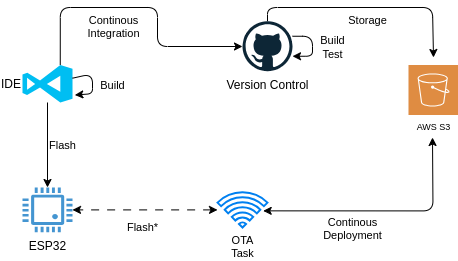
\includegraphics[width=0.5\textwidth]{architecture.png}
    \caption{System Architecture}
    \label{fig:architecture}
\end{figure}

By adopting OTA, CI/CD, and cloud-based updates, robotic swarms gain the agility required to adapt to new challenges rapidly, reflect real-time improvements, and achieve true scalability. Figure \ref{fig:architecture} shows the implementation of our system to enable over the air updates (OTA) and continuous integration \& continuous deployment (CI/CD) framework over the swam. 
\begin{itemize}
    \item \textbf{Local Development Environment}: ESP32 application development takes place locally using VSCode, the IDE environment uses version 5.2.2 of ESP-IDF and Python 3.11 to build and flash the code in-situ to the ESP32 module. This self contained development environment allows for testing new features and updates without affecting previous versions of the application running on the swarm.
    \item \textbf{Version Control System \& CI/CD}: The codebase is stored in a public repository on GitHub: \url{https://github.com/yallico/robotics_dissertation}, this allows for version control and automates the build and test process upon every commit. The ESP32 project is compiled and it generates the .bin binary file used for OTA. This process ensures that the codebase is always in a working state and ready for deployment.
    \item \textbf{Cloud Storage}: Once the OTA binary file is generated, it is uploaded to an AWS S3 public bucket. S3 serves as a reliable and low cost storage solution for the OTA updates. We decided to leave encryption and access control out of scope from the OTA implementation, yet we acknowledge that encryption is a non-trivial task that swarms should consider when deploying OTA updates in terms of computational resources required and security implications in industry. %TODO: Add reference to encryption in OTA
    \item \textbf{OTA Update Process}: The ESP32, runs a task that is triggered upon initialisation which compares its current application version against the latest version available in S3. If the version in AWS S3 diverges from the current version running in the ESP32. It then downloads the .bin file and performs the update following OTA best practice (see Section X). %TODO: Add reference to OTA best guidance from ESP-IDF.

\end{itemize}


\section{Experimental Setup}
\lipsum[5-6] % Replace with your content

\section{Notes}
Why use ESP-IDF over Arduino IDE in this project? \cite{esp-boards_esp-idf_nodate}\cite{expressif_freertos_nodate}

As we are using a ESP32 microcontroller to build our swarm, which left us with two options to program it: Arduino IDE or ESP-IDF. The reasons we chose the latter are because, first, it is the official development framework for the ESP32 microcontrollers, this means that ESP-IDF is native to ESP32 whereas Arduino is an API wrap around ESP-IDF. Making ESP-IDF more stable and enabling more advanced features, specially for communication data links such as Bluetooth, Wifi and LORA. Secondly, it is more powerful and flexible than Arduino IDE, because it allows the use of FreeRTOS which allows multi core development support (our M5 Stack has two cores) and is a pre-requisite for running microROS in the ESP32 microcontroller (at the time of writing this microROS does not support Arduino), hence making it more suitable for complex projects like this one. Thirdly, it is more efficient in terms of memory and speed (as it enables parallel processing) which is important for a project that requires real-time communication between multiple devices in a swarm. Finally, it is more professional and an industry standard, it allows dependency tracking, Over the Air (OTA) updates, unit testing, enhanced debugging and comprehensive documentation around it, which means it is more likely to be supported in the future and software is less likely to become deprecated over time.

% Add more chapters as needed

\newpage
\printbibliography

\end{document}